\section{今后工作}

\subsection{多集群CPU}

    \begin{frame}{多集群CPU分布式训练}
    \begin{block}{}
    深度神经网络模型的训练过程一般可分为前向计算(Forward)、误差反向传播(Loss Backpropagation)和参数更新。其中前向计算和反向传播的计算量很大,而且可以针对不同的训练数据进行同步计算,因此深度神经网络模型的训练过程在结构上很适合进行分布式训练。
    \end{block}
    \begin{figure}
    \centering
    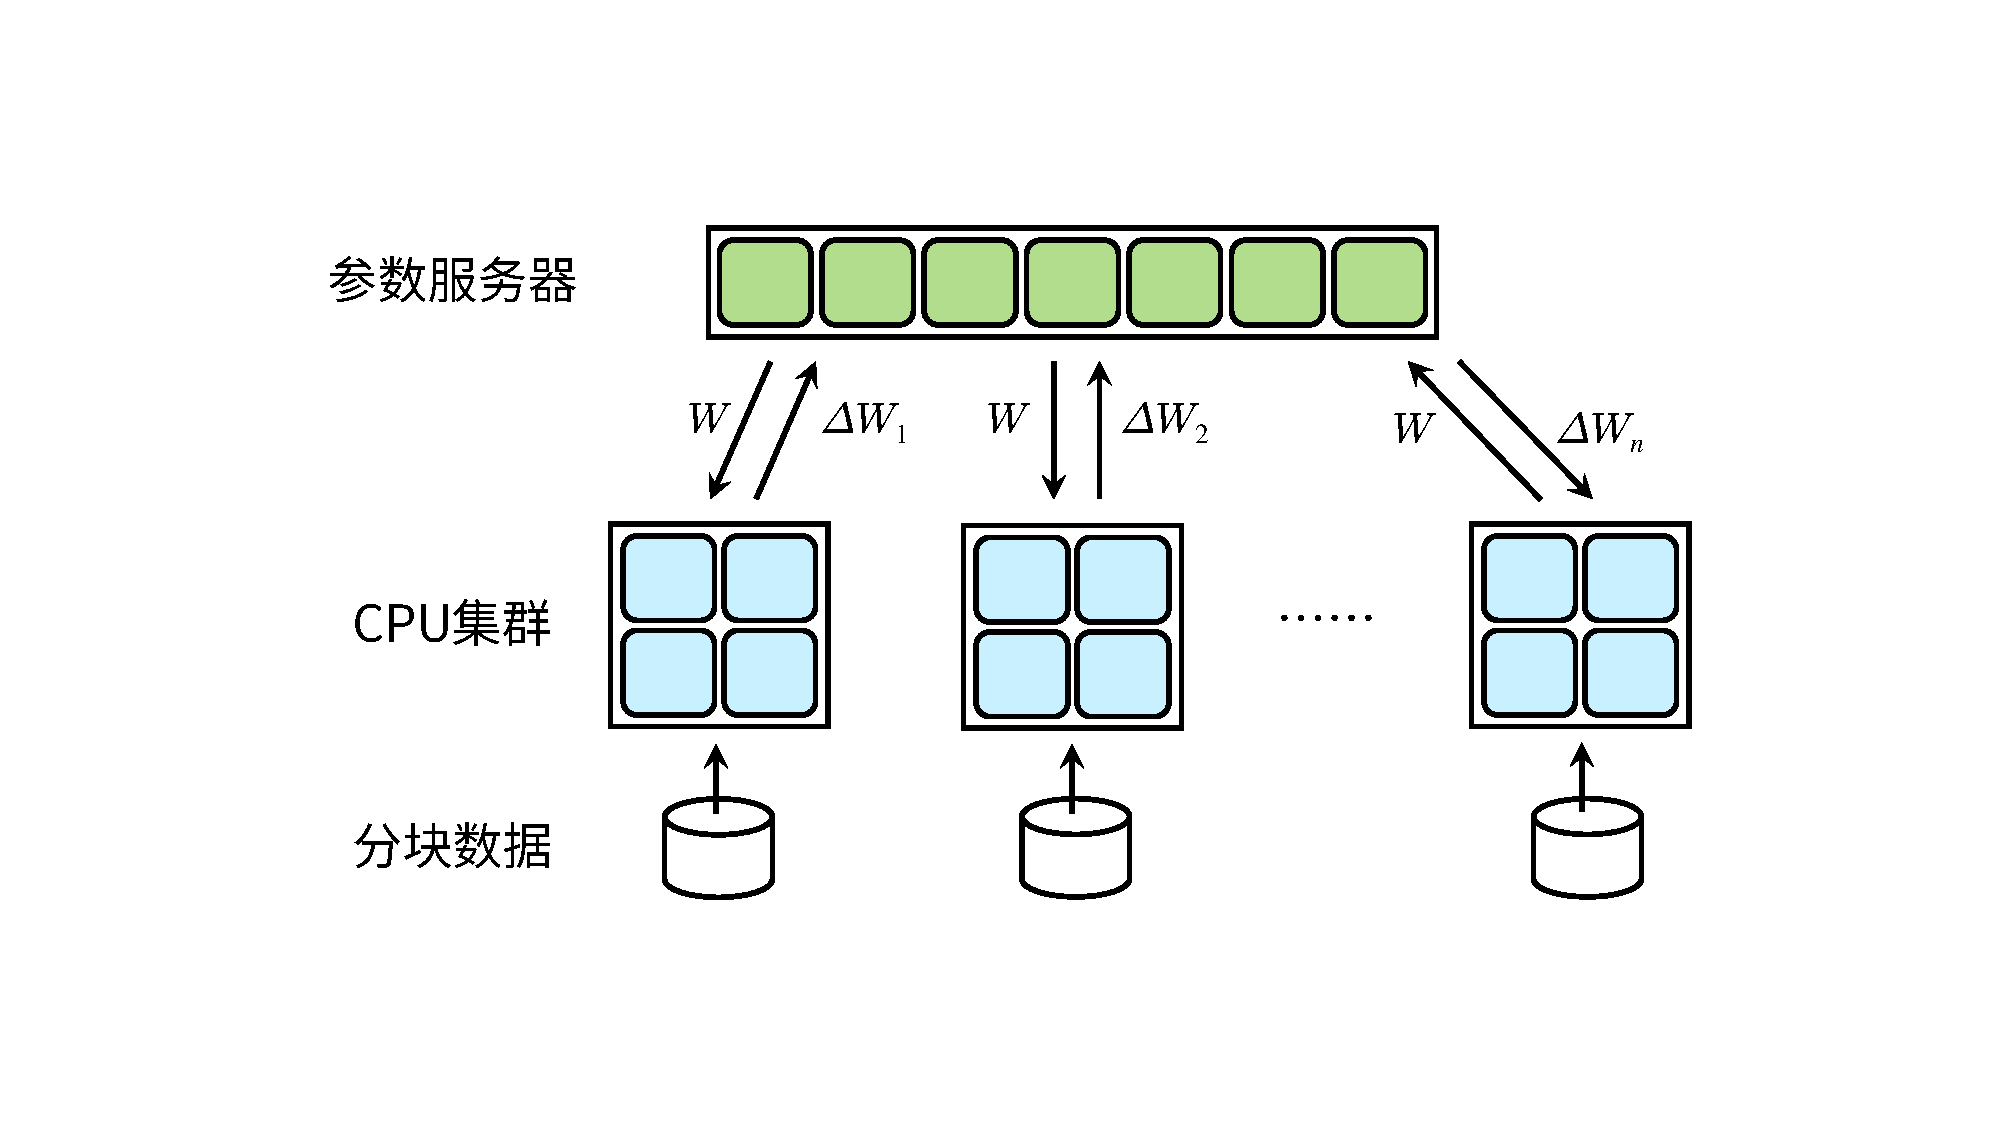
\includegraphics[width=0.5\textwidth]{figures/dist}
    \caption{分布式神经网络训练架构图}
    \label{fig:dist}
    \end{figure}
    \end{frame}

\subsection{文献翻译 + 论文写作}

    \begin{frame}{文献翻译 + 论文写作}
    \begin{block}{}
    当前进度:
    \begin{enumerate}
        \item 文献翻译 40\%
        \item 论文写作 60\%
    \end{enumerate}
    \end{block}
    \end{frame}